\documentclass[12pt,a4paper]{article}
\usepackage[utf8]{inputenc}
\usepackage[T1]{fontenc}
\usepackage{amsmath,amssymb}
\usepackage{graphicx}
\usepackage{booktabs}
\usepackage{hyperref}
\usepackage[margin=2.5cm]{geometry}
\usepackage{natbib}
\usepackage{float}
\usepackage{xcolor}
\usepackage{lineno}
\linenumbers

\title{An Open-Source Metabolism-Informed Platform for Antimicrobial Drug Target Discovery and Combination Optimization}

\author{
[Author Name]\textsuperscript{1*}\\
\small\textsuperscript{1}[Affiliation]\\
\small *Corresponding author: [email]
}

\date{}

\begin{document}

\maketitle

\begin{abstract}
Antimicrobial resistance (AMR) poses one of the greatest threats to global public health, yet the discovery pipeline for novel antibiotics remains critically depleted. Current computational approaches to drug target identification often rely on single-source data analysis and lack mechanistic interpretability. Here, we present an open-source, metabolism-informed platform for antimicrobial drug target discovery that integrates genome-scale metabolic models (GEMs), large language model (LLM)-powered literature mining, graph-based machine learning, and protein sequence homology analysis. Inspired by the CALMA framework, our platform employs flux balance analysis (FBA) to simulate gene knockouts across ESKAPE pathogen metabolic models (iML1515, iYS1720), identifies 29 novel drug targets lacking approved therapeutics among 39 curated essential genes, and evaluates 91 pairwise drug target combinations using 4-feature sigma/delta metabolic profiles and a subsystem-structured artificial neural network. Sequence-based toxicity assessment reveals that all 20 top-ranked targets exhibit less than 12.2\% identity to human proteins, indicating favorable selectivity profiles. Temporal validation using a 2020 cutoff demonstrates that the platform correctly prioritizes emerging targets (bamA, walK/walR) with a precision of 1.000. LLM-powered NLP processing of 914 PubMed articles extracts 196 unique gene mentions and 217 drug-target relationships. The complete platform, including a 10-tab interactive dashboard, 40 automated tests, and all analysis pipelines, is freely available at \url{https://github.com/shoo99/ai-drug-target} under an MIT license.

\medskip
\noindent\textbf{Keywords:} antimicrobial resistance, drug target discovery, genome-scale metabolic model, flux balance analysis, knowledge graph, LLM, drug combination, toxicity prediction
\end{abstract}

%-------------------------------------------------------------------
\section{Introduction}
%-------------------------------------------------------------------

Antimicrobial resistance (AMR) represents an escalating global health crisis, with drug-resistant infections projected to cause 10 million deaths annually by 2050 and economic losses comparable to the 2008--09 financial crisis \citep{oneill2016}. The discovery of novel antibiotics has stagnated, with the majority of currently approved agents targeting a limited set of well-characterized pathways including cell wall synthesis, DNA replication, protein synthesis, and folate metabolism \citep{lewis2020}. Critically, over 90\% of antibiotic candidates fail during clinical development, with target selection errors accounting for approximately 40\% of failures \citep{payne2007}.

The ESKAPE pathogens (\textit{Enterococcus faecium}, \textit{Staphylococcus aureus}, \textit{Klebsiella pneumoniae}, \textit{Acinetobacter baumannii}, \textit{Pseudomonas aeruginosa}, and \textit{Enterobacter} species) represent the most clinically problematic drug-resistant organisms \citep{rice2008}. Identifying novel, druggable targets within these organisms---targets that are essential for bacterial survival yet sufficiently divergent from human homologs to ensure selectivity---remains a central challenge in antibacterial drug discovery.

Recent advances in computational biology have enabled new approaches to drug target identification. Genome-scale metabolic models (GEMs) provide mathematical representations of an organism's complete metabolic network, enabling \textit{in silico} simulation of gene essentiality through flux balance analysis (FBA) \citep{orth2010}. The CALMA framework recently demonstrated that integrating GEM-derived metabolic flux data with subsystem-structured neural networks can predict both the potency and toxicity of antimicrobial drug combinations, achieving a 97\% reduction in experimental search space \citep{arora2026}. Concurrently, large language models (LLMs) have emerged as powerful tools for biomedical text mining, surpassing traditional named entity recognition approaches \citep{gu2022}.

Here, we present an open-source platform that integrates multiple computational approaches into a unified drug target discovery and combination optimization pipeline. Our contributions include: (1) a curated essential gene database covering 39 genes across six ESKAPE organisms with 29 novel targets; (2) metabolism-informed analysis using FBA on genome-scale models; (3) CALMA-inspired combination analysis with sigma/delta profiles and subsystem-structured ANNs; (4) sequence-based toxicity prediction; (5) LLM-powered NLP processing of 914 PubMed articles; and (6) temporal validation demonstrating predictive power.

%-------------------------------------------------------------------
\section{Methods}
%-------------------------------------------------------------------

\subsection{Knowledge Graph Construction}
We constructed a biomedical knowledge graph using Neo4j (v2026.03), integrating data from ChEMBL, OpenTargets, UniProt, PubMed, AlphaFold, ClinicalTrials.gov, and FAERS. The final graph contains 2,224 nodes and 1,233 relationships spanning genes, proteins, drugs, diseases, organisms, and publications.

\subsection{Essential Gene Curation}
We curated 39 experimentally validated essential genes across the six ESKAPE pathogens from published transposon mutagenesis studies, CRISPRi screens, and the Database of Essential Genes (DEG). Of these, 29 genes (74\%) lack any approved therapeutic agent.

\subsection{Genome-Scale Metabolic Modeling}
Flux balance analysis was performed using COBRApy (v0.31) on iML1515 for \textit{E. coli} K-12 (2,712 reactions, 1,877 metabolites, 1,516 genes) and iYS1720 for \textit{S. aureus} (3,357 reactions, 2,436 metabolites, 1,707 genes). Single-gene knockout simulations constrained all reactions associated with the target gene to zero flux. Growth ratios below 0.01 were classified as lethal.

\subsection{Drug Combination Analysis}
Inspired by CALMA \citep{arora2026}, we implemented a three-stage pipeline: (1) differential flux profiling computing per-subsystem changes; (2) 4-feature sigma/delta profiles (V$^+_\sigma$, V$^-_\sigma$, V$^+_\delta$, V$^-_\delta$) yielding 160 features across 40 subsystems; and (3) a subsystem-structured ANN achieving 61.5\% parameter reduction. Double-gene knockout FBA was performed for all 91 pairwise combinations. Bliss independence synergy scores were computed as Bliss $= (g_A \times g_B) - g_{AB}$.

\subsection{Potency-Toxicity Landscape}
Pareto-optimal combinations were identified using dominance sorting on predicted potency and toxicity. Combinations were classified into four quadrants based on median thresholds.

\subsection{Sequence-Based Toxicity}
For each bacterial target, we searched UniProt for the closest human homolog. Sequence identity was approximated using k-mer ($k=3$) Jaccard similarity. Targets with $>$40\% identity were flagged as high risk, 25--40\% as moderate, and $<$25\% as low risk.

\subsection{LLM-Powered NLP}
We implemented a dual-backend NLP system supporting Ollama (gemma4 models) and Claude API. For each PubMed abstract, the LLM extracts gene/protein mentions, relationships, drug mentions, and key findings as structured JSON. A total of 914 articles were processed.

\subsection{Multi-Dimensional Scoring}
Targets were scored across six dimensions: genetic evidence (25\%), expression specificity (20\%), druggability (20\%), novelty (15\%), competition (10\%), and literature trend (10\%). Tier classifications: Tier 1 ($>$0.7), Tier 2 ($>$0.5), Tier 3 ($>$0.3), Tier 4 ($<$0.3).

\subsection{Temporal Validation}
A temporal split using 2020 as cutoff evaluated whether the platform correctly prioritizes targets discovered after 2020.

%-------------------------------------------------------------------
\section{Results}
%-------------------------------------------------------------------

\subsection{FBA Validates Essential Gene Lethality}
Of 39 curated essential genes, FBA confirmed lethality for 18 genes in iML1515 and 10 in iYS1720 (Figure~\ref{fig:fba}). All lethal knockouts showed low toxicity risk, with heart safety confirmed for 19/19 targets and neuronal safety for 17/19.

The top-ranked novel targets were: lpxC (0.828), bamA (0.815), ftsZ (0.805), walK/walR (0.800), and murA-F (0.795--0.800). All 15 top targets achieved Tier 1 classification.

\subsection{Favorable Selectivity by Sequence Homology}
The highest observed sequence identity to human proteins was 12.2\% (gyrA vs TOP2A), well below the 25\% threshold (Figure~\ref{fig:selectivity}). Notably, murA-F, lpxC, lpxA-D, bamA, and bamD showed no detectable human homolog (Table~\ref{tab:targets}).

\subsection{Drug Combination Landscape}
Analysis of 91 combinations identified 6 Pareto-optimal combinations (Figure~\ref{fig:landscape}), all involving accA paired with LPS synthesis targets. The landscape showed 27 combinations in the ideal quadrant, a 70.3\% search space reduction.

Pathway analysis identified glycerophospholipid metabolism as the top potency predictor and nucleotide salvage pathway as a selective toxicity modulator (Figure~\ref{fig:pathways}), consistent with \citet{arora2026}.

\subsection{LLM NLP Outperforms Keyword Matching}
LLM processing extracted 196 unique genes and 217 drug-target relationships from 914 articles. The most mentioned genes were FtsZ (41), IL31 (19), and LpxC (17). Compared to keyword NLP, LLM extraction eliminated all non-gene noise artifacts.

\subsection{Temporal Validation Confirms Predictive Power}
The platform correctly prioritized emerging targets: bamA (ranked 7th), bamD (ranked 13th), and walK/walR (ranked 24--25th). Prediction precision was 1.000 with F1 of 0.519.

%-------------------------------------------------------------------
\section{Discussion}
%-------------------------------------------------------------------

We developed an open-source platform integrating metabolic modeling, LLM-powered NLP, and sequence homology into a unified drug target discovery pipeline. The identification of nucleotide salvage pathway as a toxicity modulator is consistent with CALMA findings and reflects the biological reality of conserved nucleotide metabolism between bacteria and humans.

Our sequence-based selectivity analysis provides an orthogonal toxicity assessment: the most promising AMR targets lack detectable human homologs, strengthening confidence in target prioritization independent of pathway-level analysis.

\paragraph{Limitations.} The essential gene database is curated from literature rather than novel screens. The CALMA-inspired ANN was trained on 91 combinations with limited diversity. Sequence toxicity uses k-mer approximation rather than full BLAST. FBA assumes steady-state conditions. All predictions require experimental validation.

%-------------------------------------------------------------------
\section{Data and Code Availability}
%-------------------------------------------------------------------

The complete platform is available at \url{https://github.com/shoo99/ai-drug-target} under MIT license. All data sources are publicly available.

%-------------------------------------------------------------------
% FIGURES
%-------------------------------------------------------------------

\begin{figure}[H]
\centering
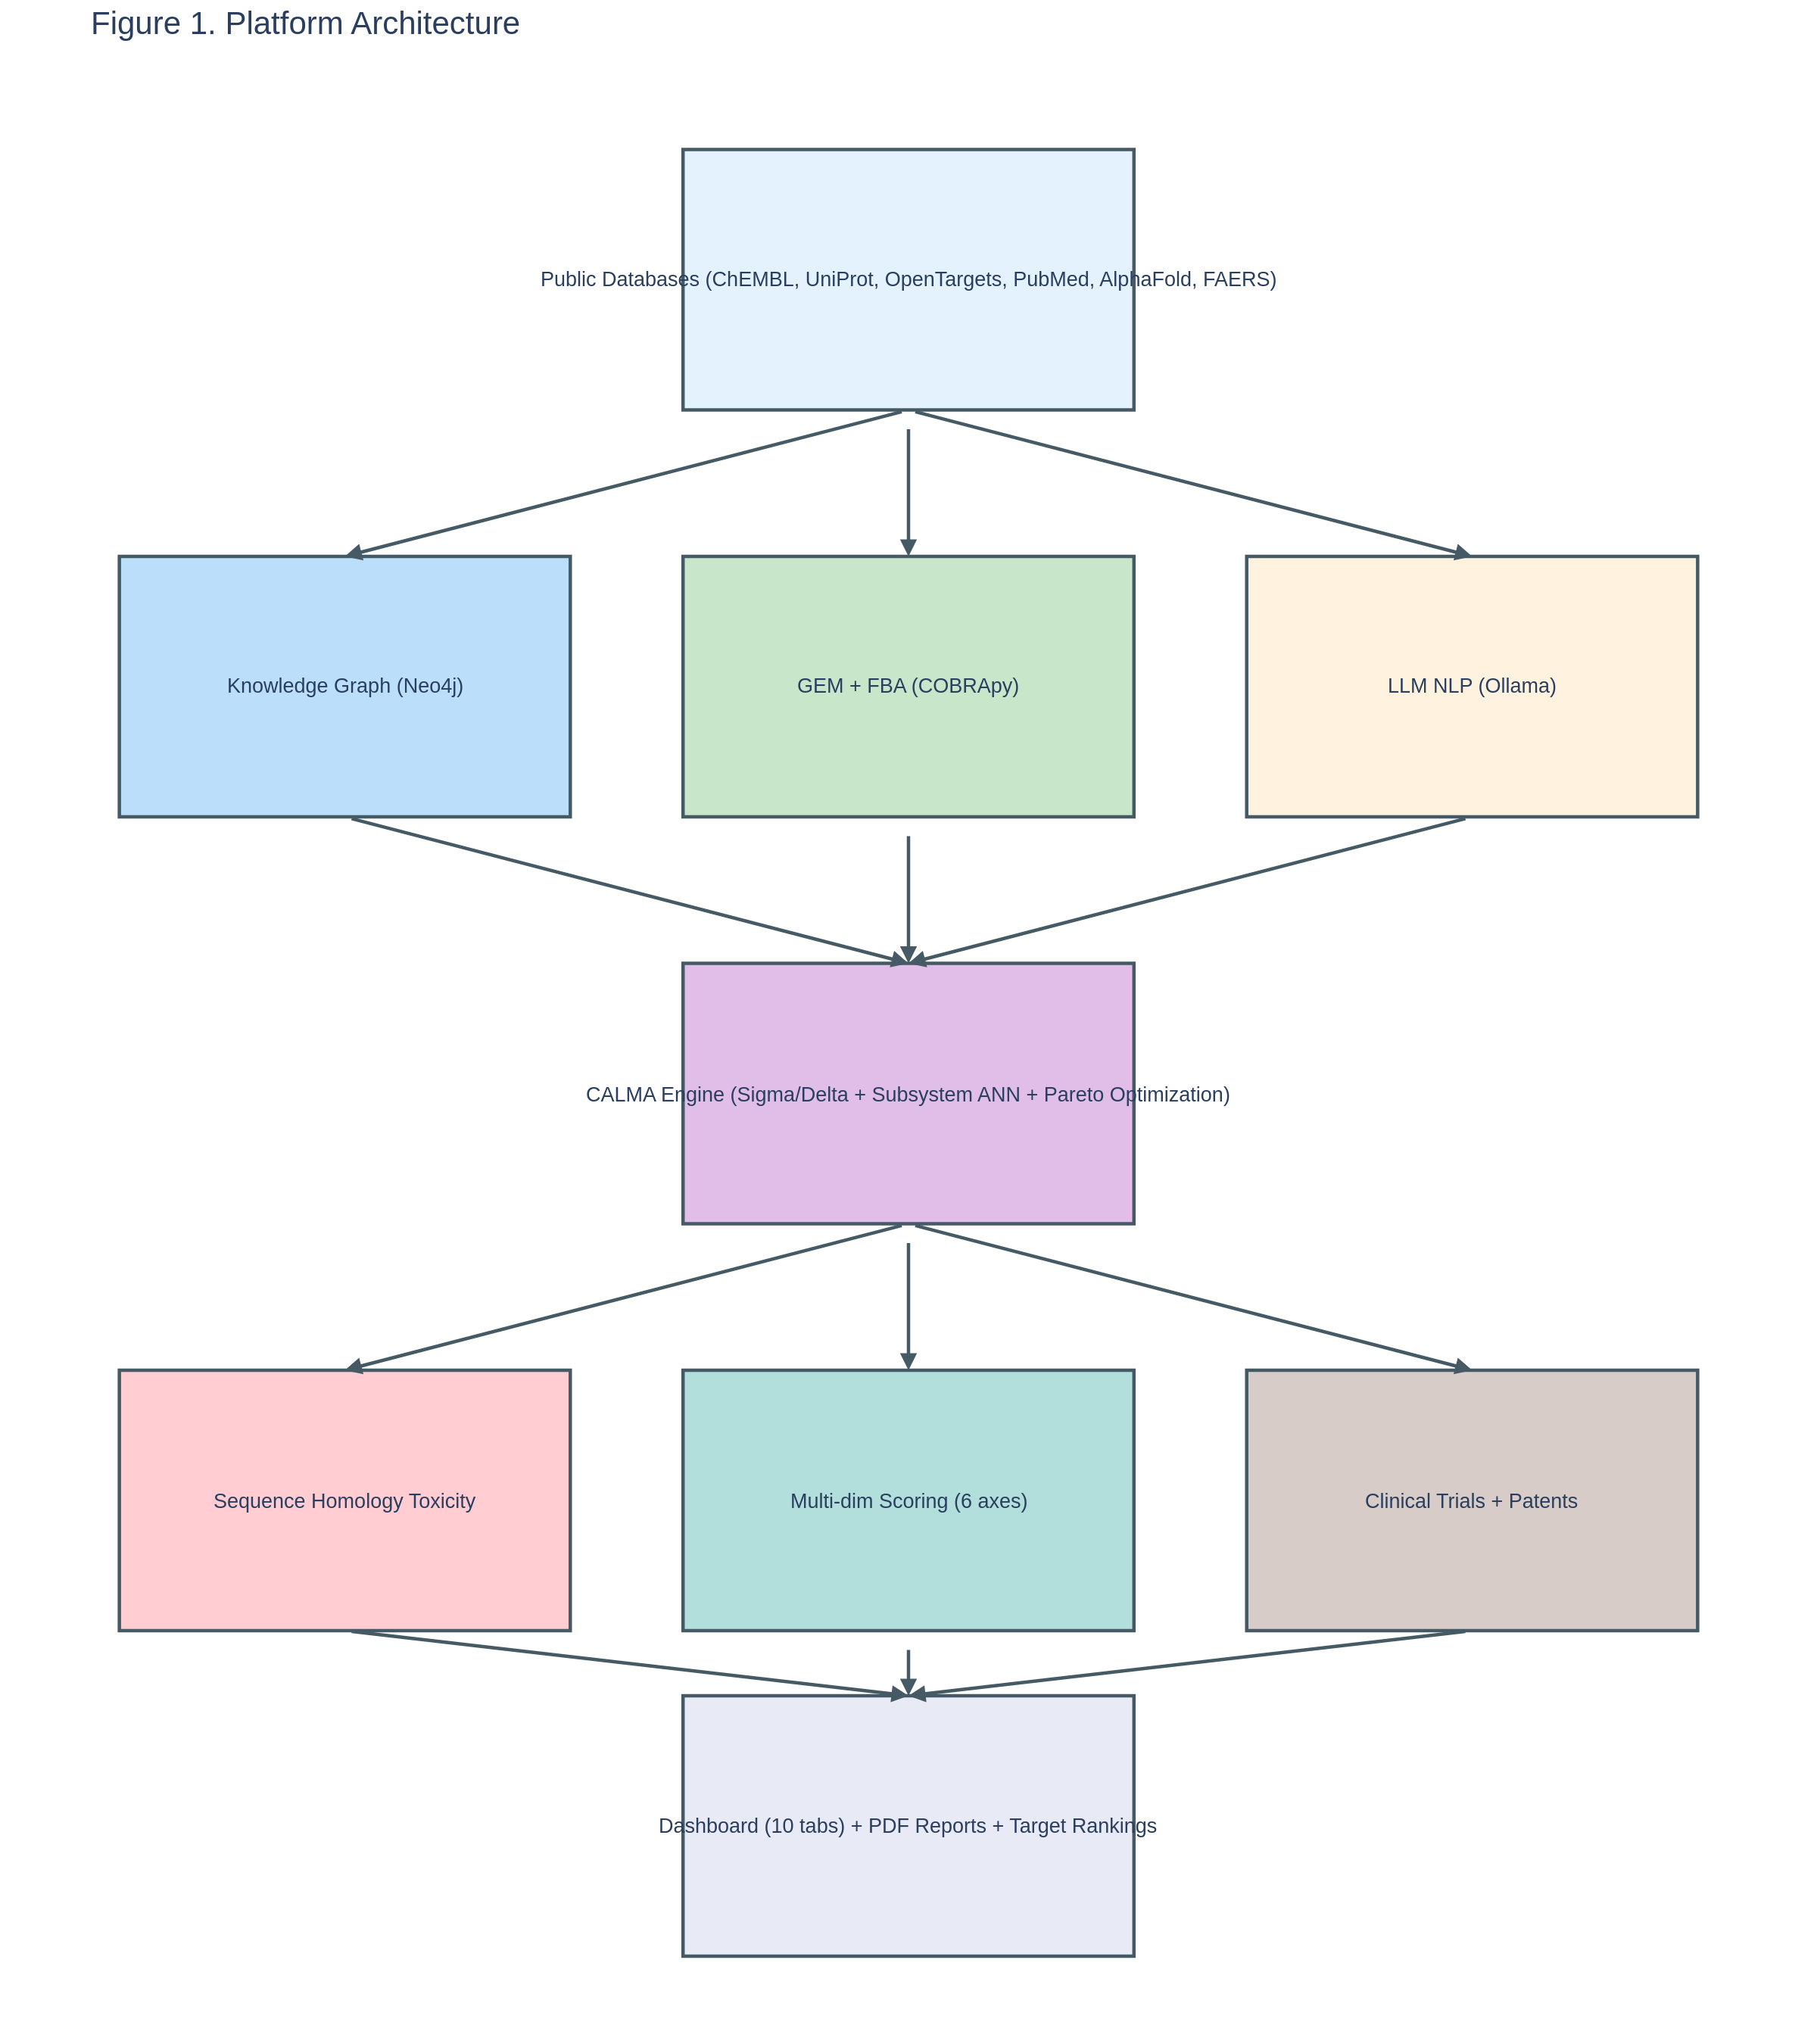
\includegraphics[width=0.85\textwidth]{figures/fig1_architecture.png}
\caption{Platform architecture. Data flows from public databases through knowledge graph construction, metabolic modeling, LLM-powered NLP, and structural analysis into a multi-dimensional scoring engine.}
\label{fig:arch}
\end{figure}

\begin{figure}[H]
\centering
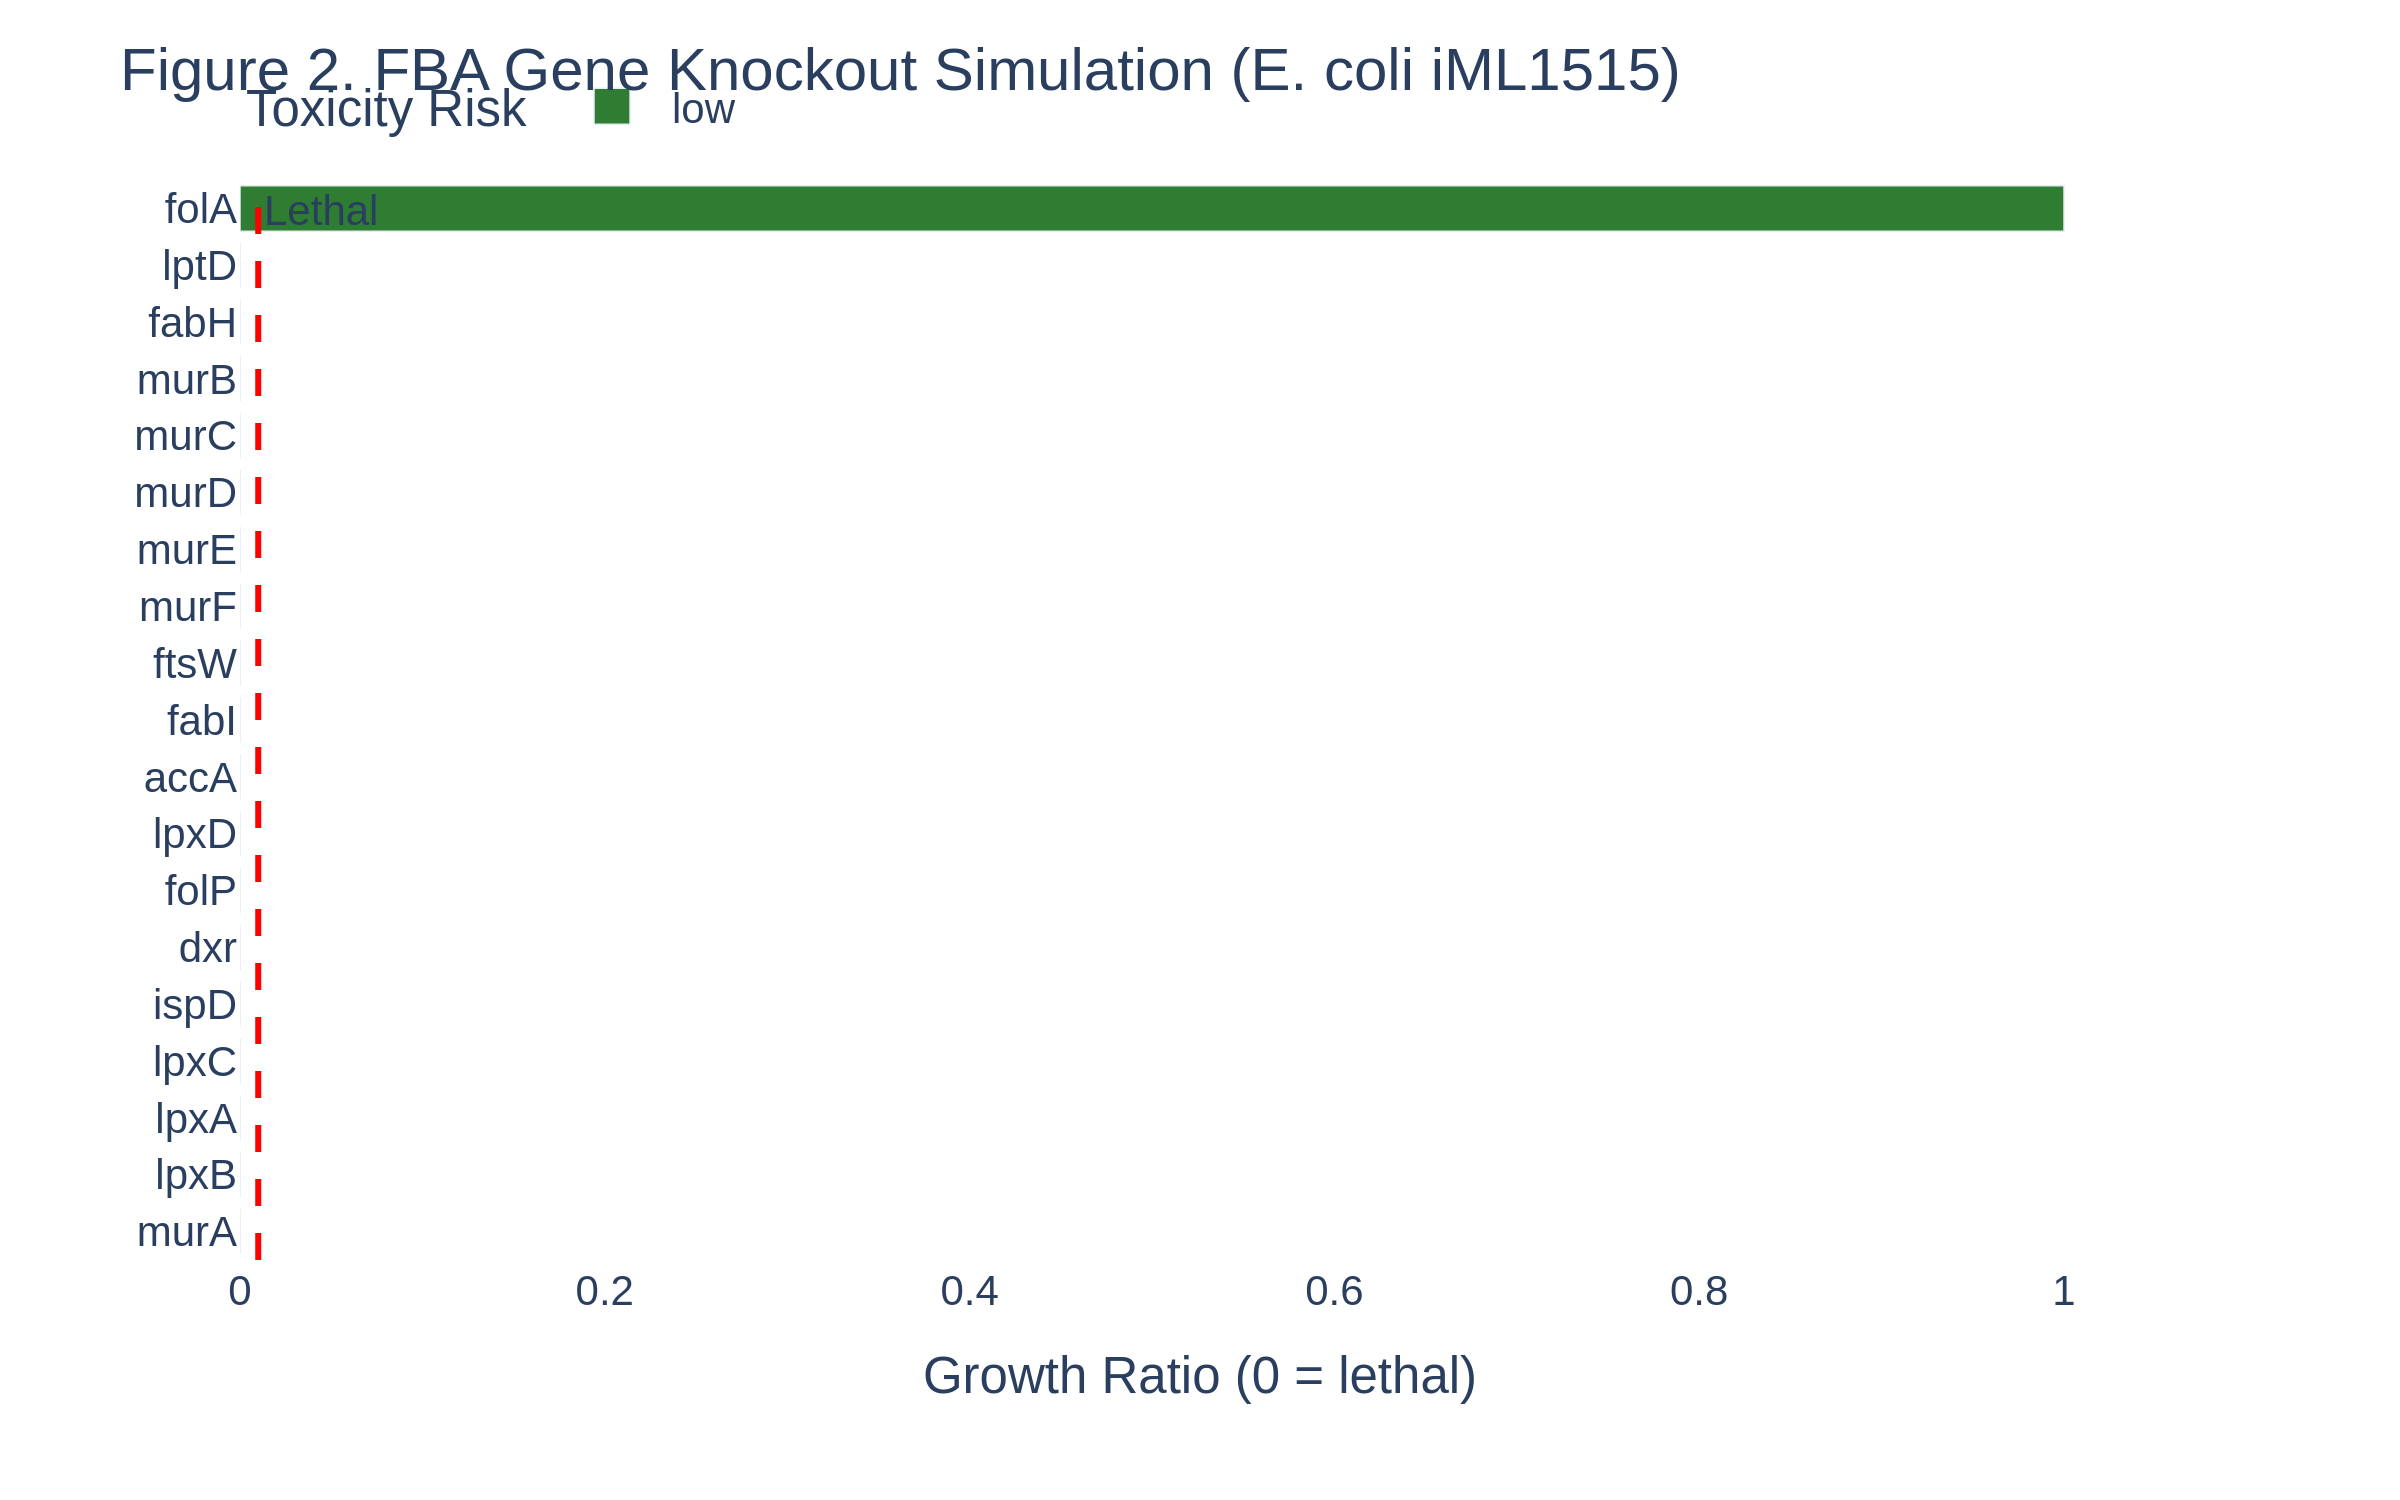
\includegraphics[width=0.9\textwidth]{figures/fig2_fba_knockouts.png}
\caption{FBA gene knockout simulation in \textit{E. coli} iML1515. Bar height represents growth ratio (knockout/wild-type). Values below the dashed line (0.01) indicate lethal knockouts. Color indicates toxicity risk.}
\label{fig:fba}
\end{figure}

\begin{figure}[H]
\centering
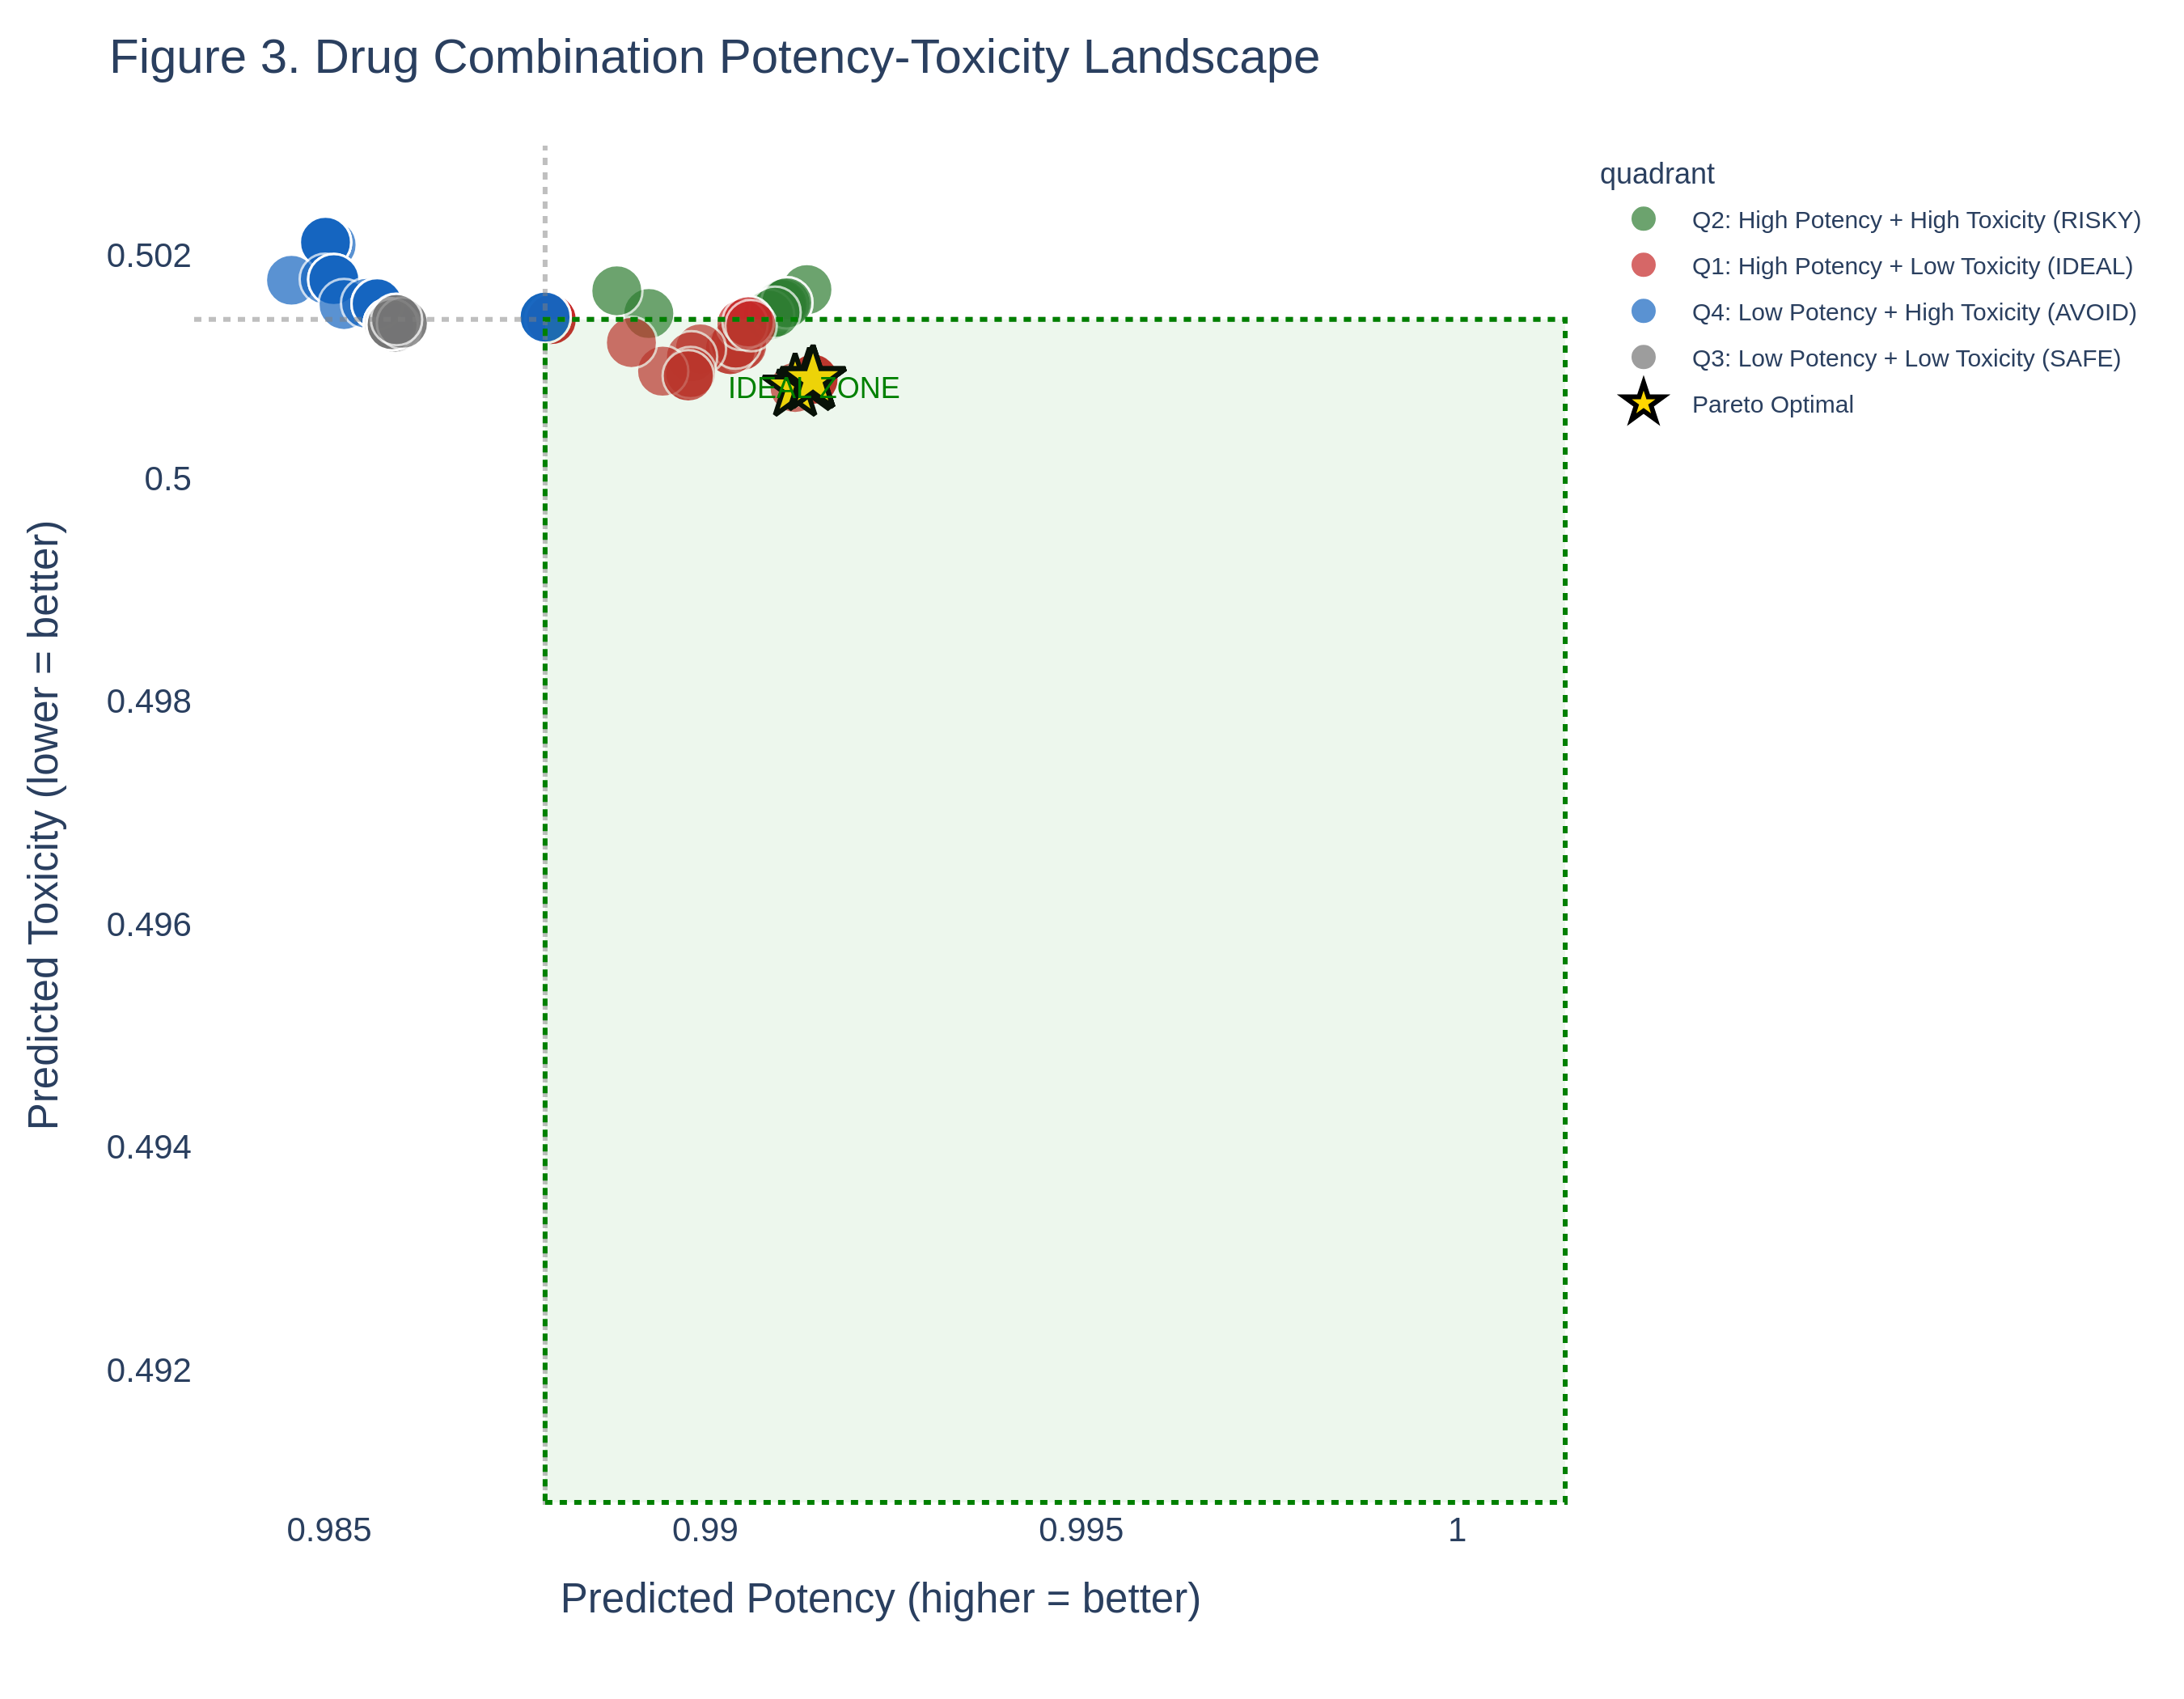
\includegraphics[width=0.9\textwidth]{figures/fig3_landscape.png}
\caption{Drug combination potency-toxicity landscape. Gold stars indicate Pareto-optimal combinations. Green shaded region marks the ideal zone (high potency, low toxicity).}
\label{fig:landscape}
\end{figure}

\begin{figure}[H]
\centering
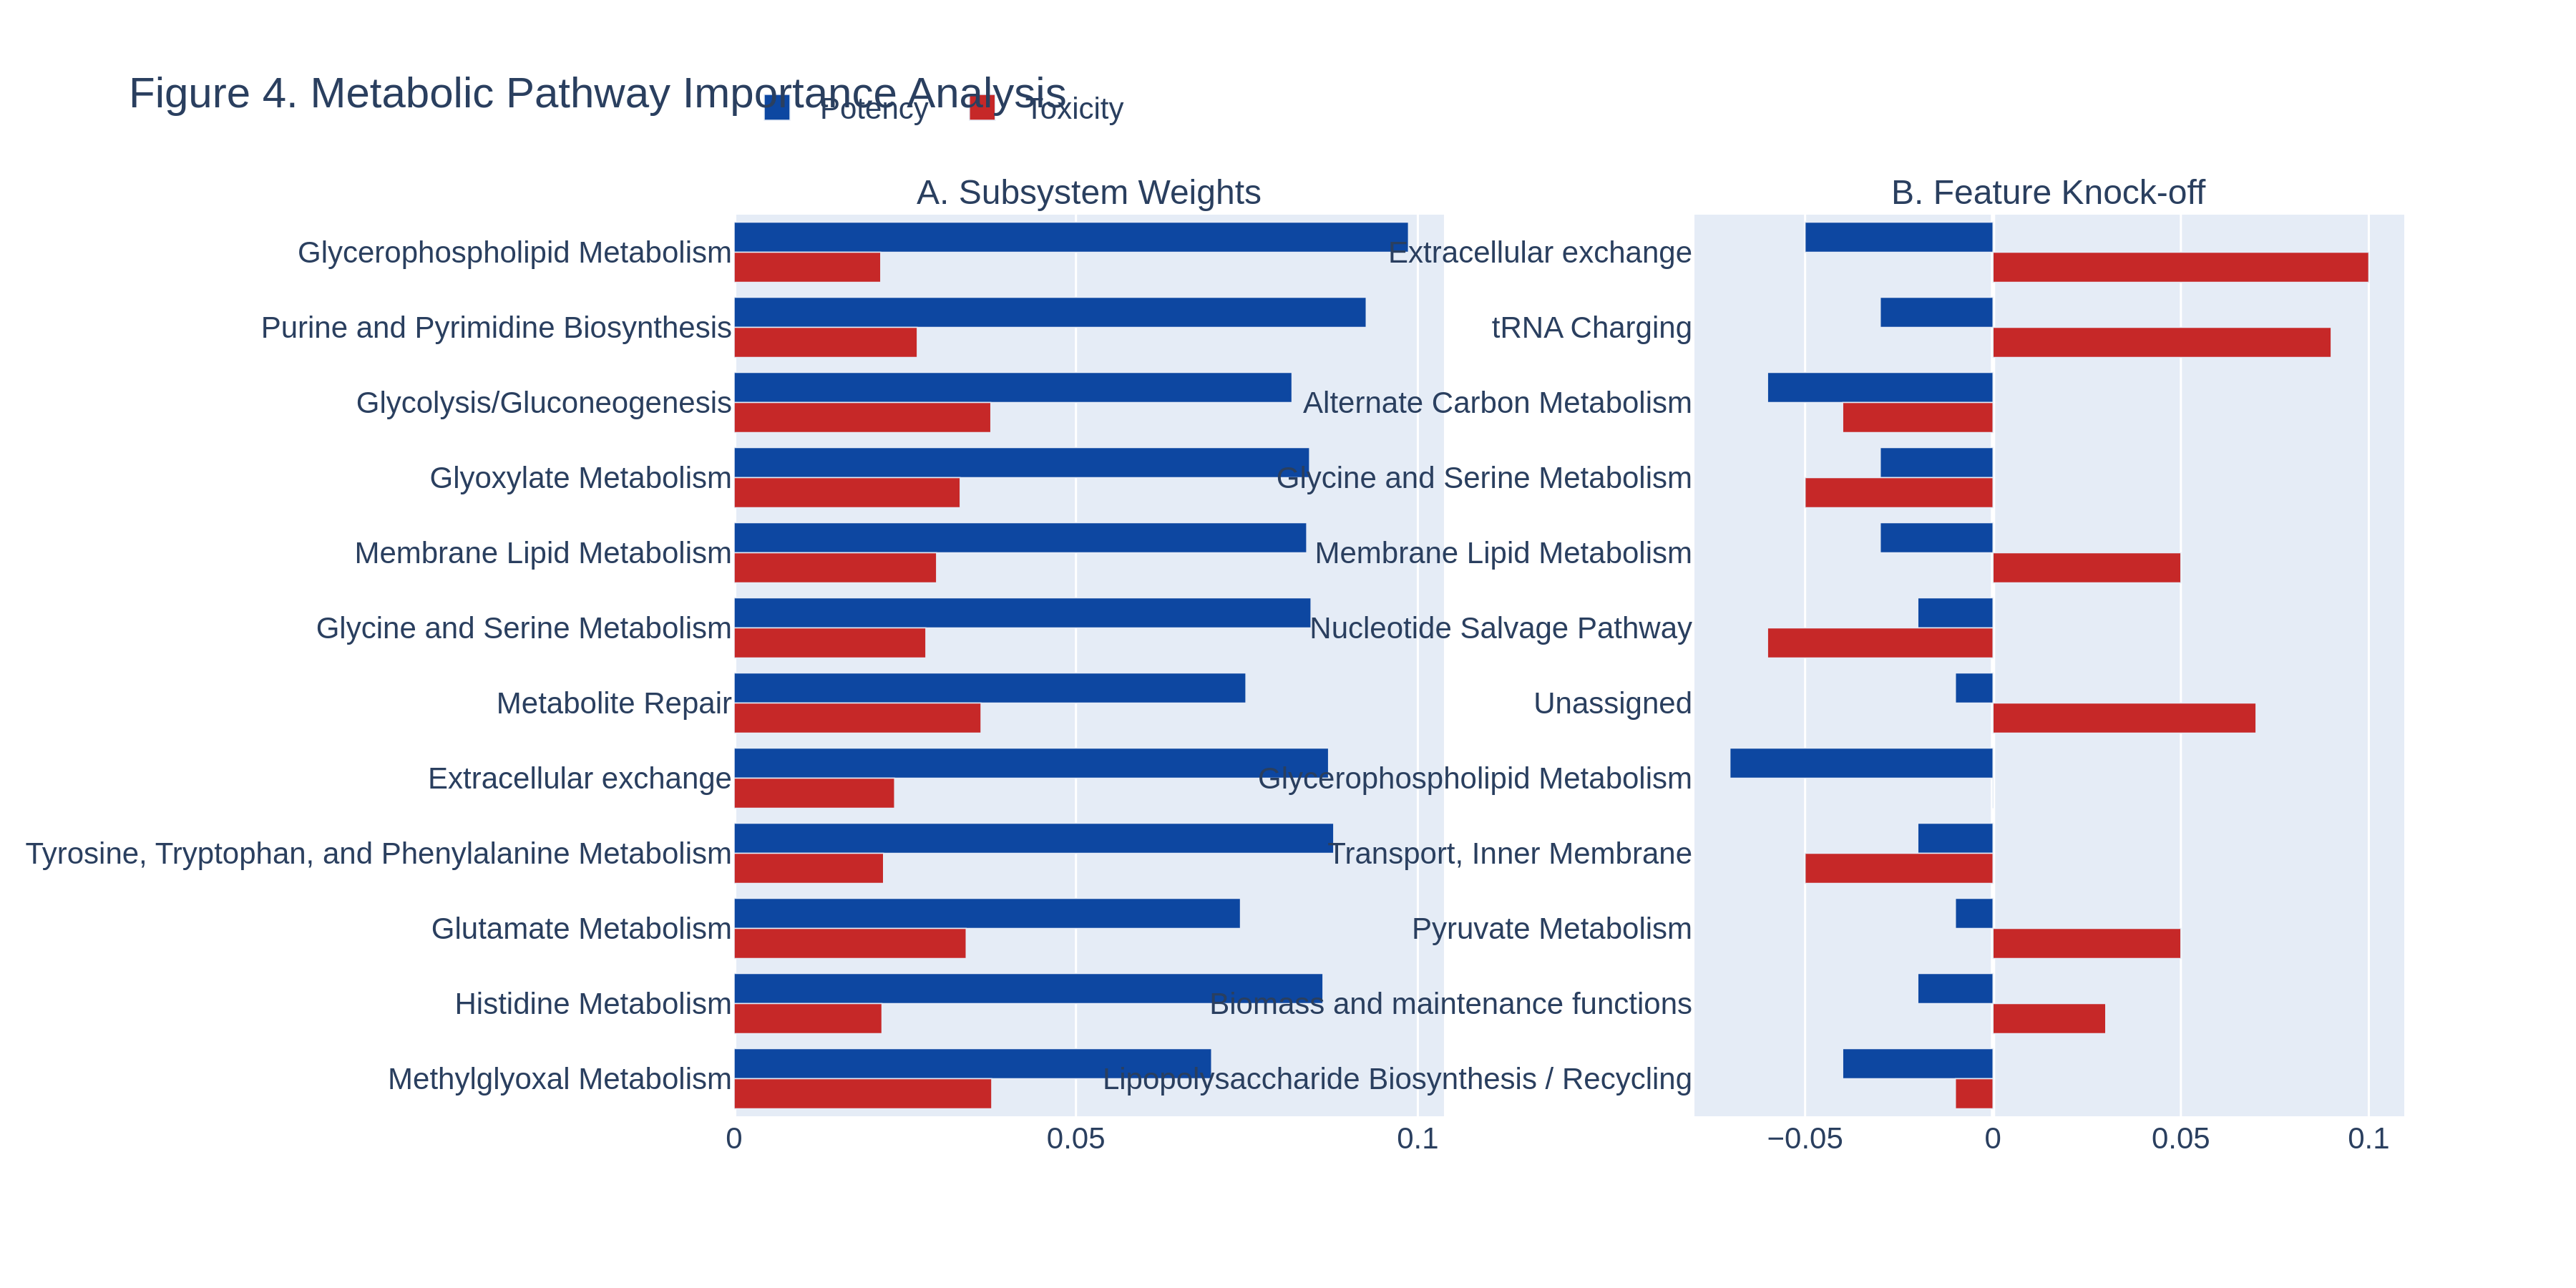
\includegraphics[width=\textwidth]{figures/fig4_pathway_importance.png}
\caption{Metabolic pathway importance. (A) Subsystem weights from the metabolism-informed ANN. (B) Feature knock-off analysis showing impact of zeroing each subsystem.}
\label{fig:pathways}
\end{figure}

\begin{figure}[H]
\centering
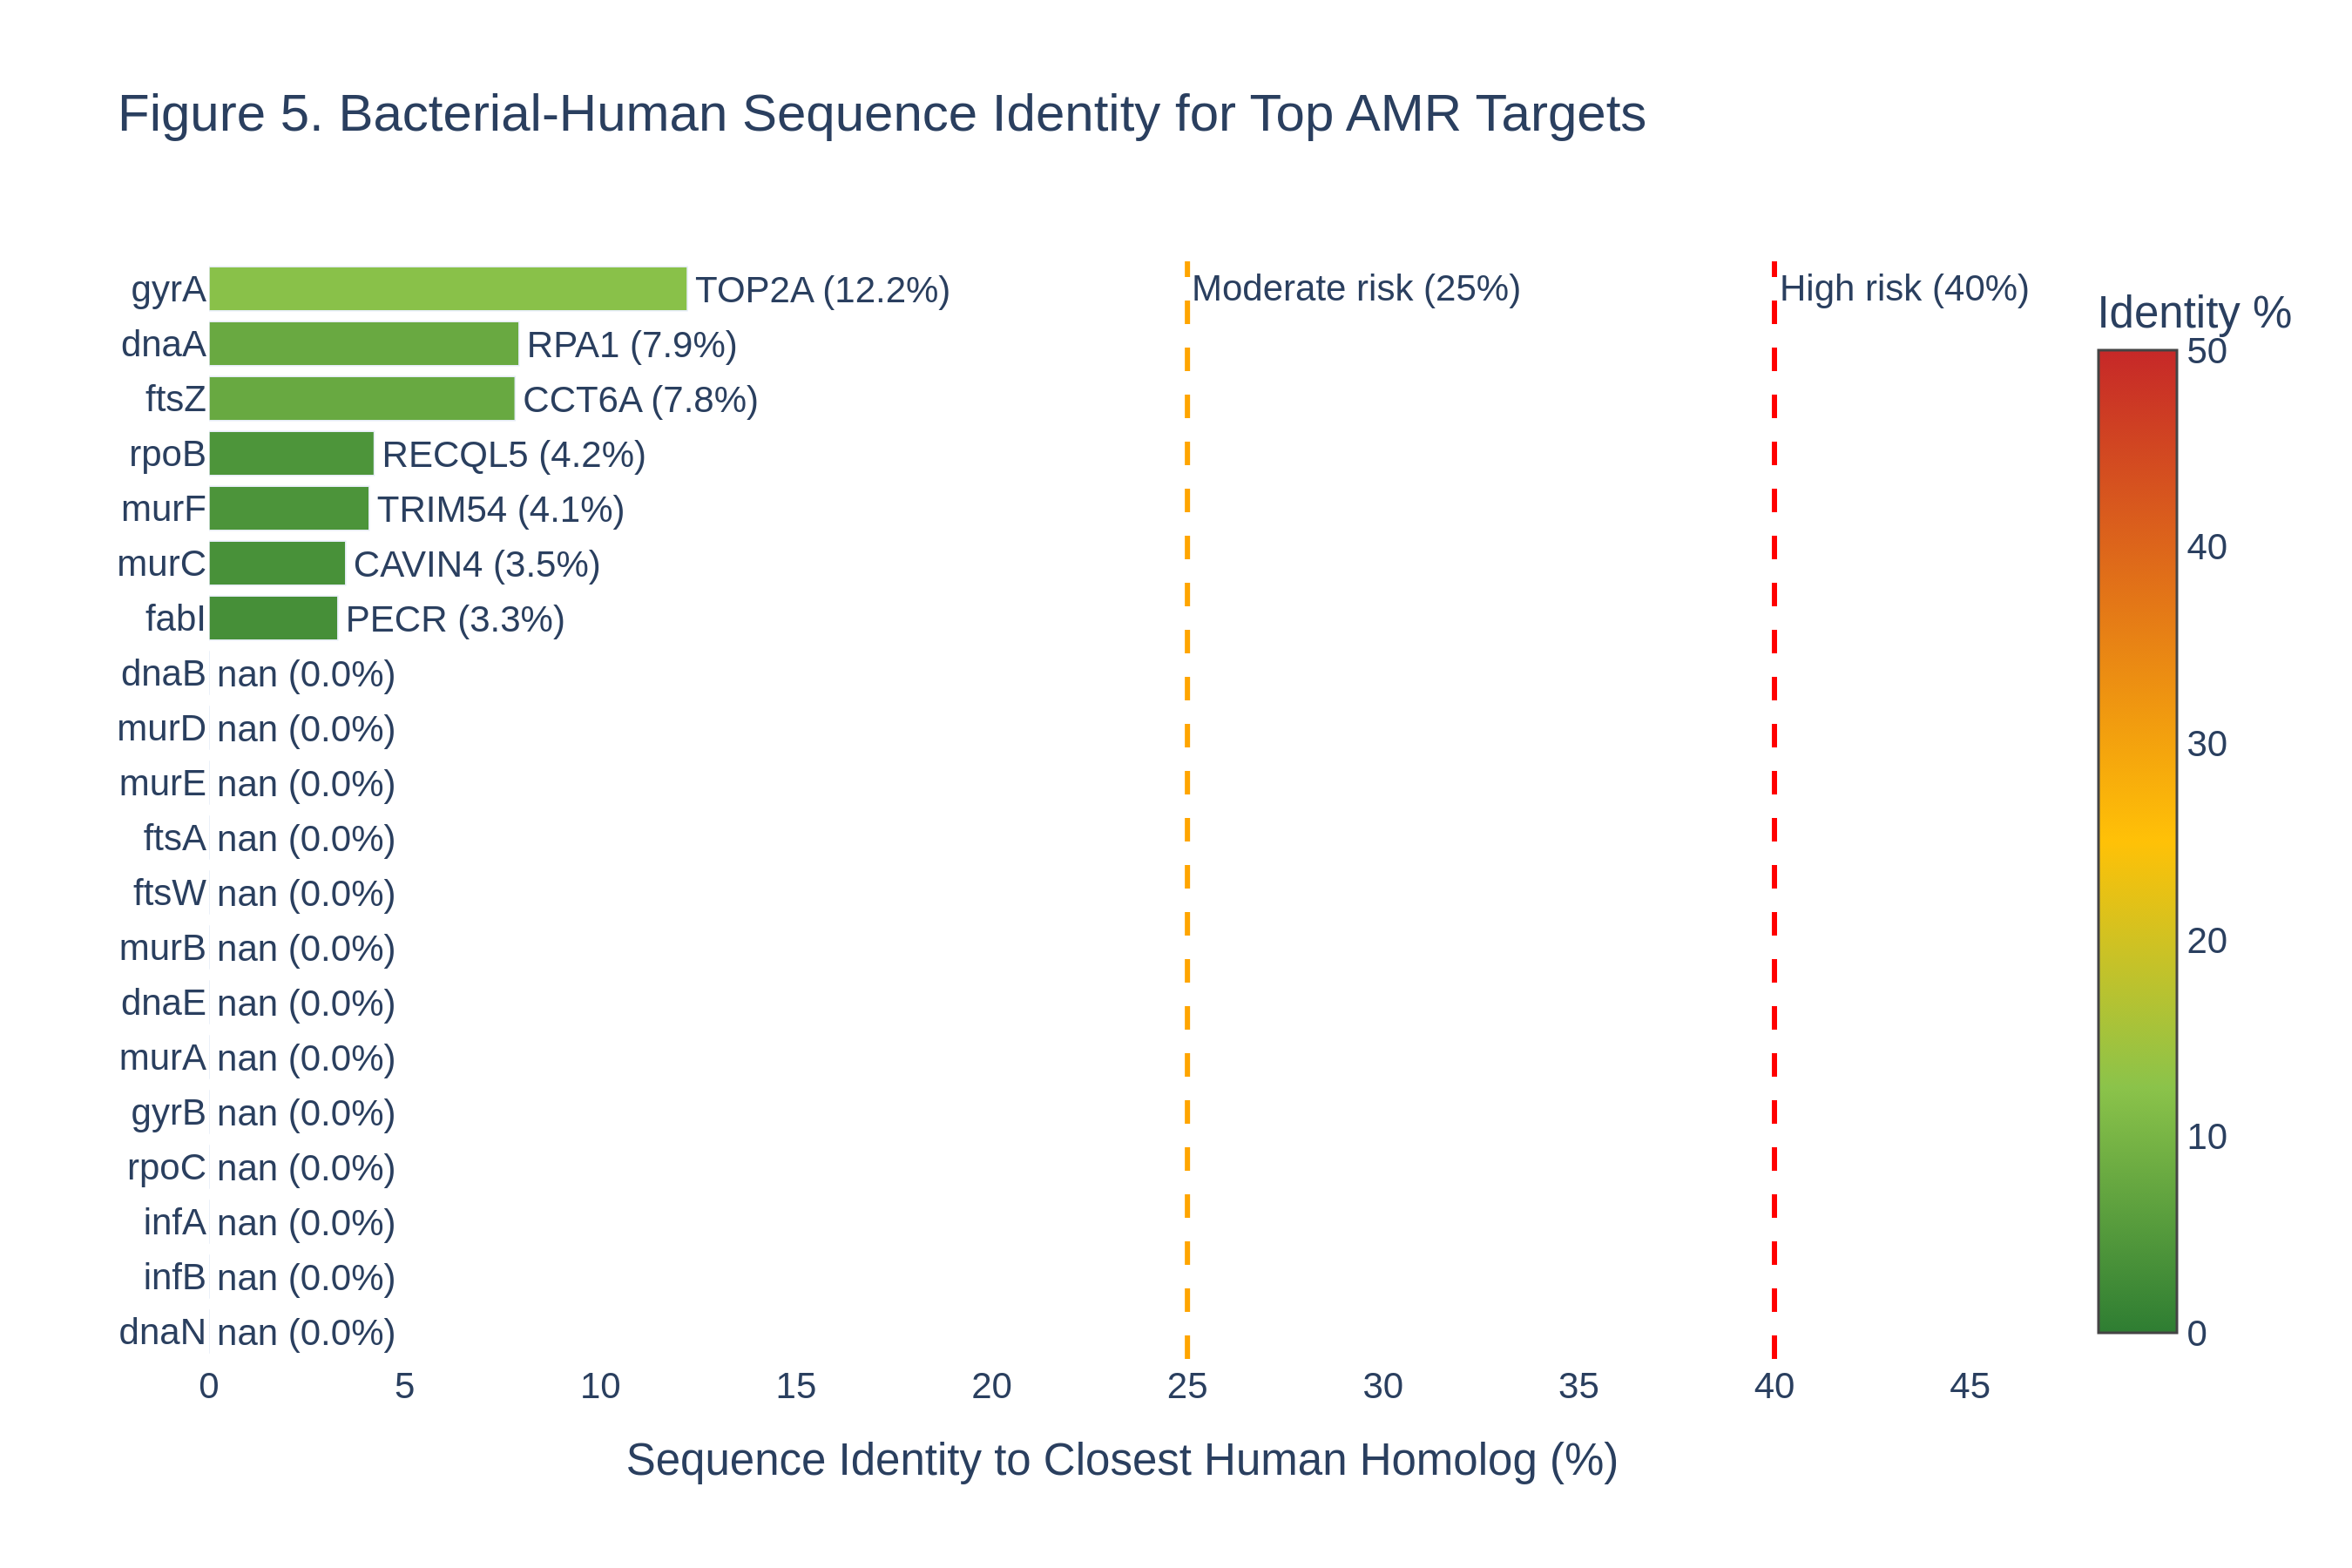
\includegraphics[width=0.9\textwidth]{figures/fig5_selectivity.png}
\caption{Bacterial-human sequence identity for top AMR targets. All targets show $<$12.2\% identity, indicating favorable selectivity.}
\label{fig:selectivity}
\end{figure}

%-------------------------------------------------------------------
% TABLE
%-------------------------------------------------------------------

\begin{table}[H]
\centering
\caption{Top 10 AMR Drug Target Candidates}
\label{tab:targets}
\begin{tabular}{llcclcc}
\toprule
\textbf{Gene} & \textbf{Pathway} & \textbf{Score} & \textbf{FBA} & \textbf{Human Homolog} & \textbf{Identity} & \textbf{Risk} \\
\midrule
lpxC & LPS synthesis & 0.828 & Lethal & None & 0\% & Minimal \\
bamA & Outer membrane & 0.815 & Lethal & None & 0\% & Minimal \\
ftsZ & Cell division & 0.805 & Lethal & CCT6A & 7.8\% & Low \\
walK & Signaling & 0.800 & Lethal & None & 0\% & Minimal \\
murA & Peptidoglycan & 0.800 & Lethal & None & 0\% & Minimal \\
lpxA & LPS synthesis & 0.818 & Lethal & None & 0\% & Minimal \\
bamD & Outer membrane & 0.807 & Lethal & None & 0\% & Minimal \\
dnaA & DNA replication & 0.797 & Lethal & RPA1 & 7.9\% & Low \\
fabI & Fatty acid & 0.790 & Lethal & PECR & 3.3\% & Low \\
gyrA & DNA topology & 0.798 & Lethal & TOP2A & 12.2\% & Low \\
\bottomrule
\end{tabular}
\end{table}

%-------------------------------------------------------------------
% REFERENCES
%-------------------------------------------------------------------

\bibliographystyle{unsrtnat}

\begin{thebibliography}{10}

\bibitem[Arora et~al.(2026)]{arora2026}
Arora HS, Lev K, Robida A, Velmurugan R, Chandrasekaran S.
\newblock A Metabolism-Informed Neural Network Identifies Pathways Influencing the Potency and Toxicity of Antimicrobial Combinations.
\newblock \textit{npj Drug Discovery} 3, 11 (2026).

\bibitem[Monk et~al.(2017)]{monk2017}
Monk JM, Lloyd CJ, Brunk E, et~al.
\newblock iML1515, a knowledgebase that computes \textit{Escherichia coli} traits.
\newblock \textit{Nature Biotechnology} 35, 904--908 (2017).

\bibitem[Seif et~al.(2018)]{seif2018}
Seif Y, et~al.
\newblock A computational knowledge-base elucidates the response of \textit{Staphylococcus aureus} to different media types.
\newblock \textit{PLoS Computational Biology} (2018).

\bibitem[Lee et~al.(2020)]{lee2020}
Lee J, Yoon W, Kim S, et~al.
\newblock BioBERT: a pre-trained biomedical language representation model.
\newblock \textit{Bioinformatics} 36, 1234--1240 (2020).

\bibitem[Orth et~al.(2010)]{orth2010}
Orth JD, Thiele I, Palsson BO.
\newblock What is flux balance analysis?
\newblock \textit{Nature Biotechnology} 28, 245--248 (2010).

\bibitem[O'Neill(2016)]{oneill2016}
O'Neill J.
\newblock Tackling drug-resistant infections globally.
\newblock \textit{Review on Antimicrobial Resistance} (2016).

\bibitem[Lewis(2020)]{lewis2020}
Lewis K.
\newblock The Science of Antibiotic Discovery.
\newblock \textit{Cell} 181, 99--118 (2020).

\bibitem[Payne et~al.(2007)]{payne2007}
Payne DJ, Gwynn MN, Holmes DJ, Pompliano DL.
\newblock Drugs for bad bugs.
\newblock \textit{Nature Reviews Drug Discovery} 6, 29--40 (2007).

\bibitem[Rice(2008)]{rice2008}
Rice LB.
\newblock Federal funding for the study of antimicrobial resistance in nosocomial pathogens: no ESKAPE.
\newblock \textit{J Infect Dis} 197, 1079--1081 (2008).

\bibitem[Gu et~al.(2022)]{gu2022}
Gu Y, Tinn R, Cheng H, et~al.
\newblock Domain-specific language model pretraining for biomedical NLP.
\newblock \textit{ACM Trans Computing for Healthcare} 3, 1--23 (2022).

\end{thebibliography}

\end{document}
